% TEMPLATE.TEX
%
% Time-stamp: <2013-03-26 11:09 olenz>
%
% This is an extensively documented LaTeX file that shows how to
% produce a good-looking document with current LaTeX (11/2012).
%
% IMPORTANT!
%
%   Some obsolete commands and packages
% ----------|-------------------------------
% obsolete  |     Replacement in LATEX 2ε
% ----------|-------------------------------
%           | local            global/switch
% ----------|-------------------------------
% {\bf ...} | \textbf{...}     \bfseries
%     -     | \emph{...}       \em
% {\it ...} | \textit{...}     \itshape
%     -     | \textmd{...}     \mdseries
% {\rm ...} | \textrm{...}     \rmfamily
% {\sc ...} | \textsc{...}     \scshape
% {\sf ...} | \textsf{...}     \sffamily
% {\sl ...} | \textsl{...}     \slshape
% {\tt ...} | \texttt{...}     \ttfamily
%     -     | \textup{...}     \upshape
%
% DON'T USE \\ TO MAKE LINEBREAKS, INSTEAD JUST LEAVE A BLANK LINE!
%
\RequirePackage[l2tabu,orthodox]{nag} % turn on warnings because of bad style
\documentclass[a4paper,10pt,bibtotoc]{scrartcl}
%
\usepackage[bottom=3.5cm, top=2cm]{geometry}
%%%%%%%%%%%%%%%%%%%%%%%%%%%%%%%%%%%%
% KOMA CLASSES
%%%%%%%%%%%%%%%%%%%%%%%%%%%%%%%%%%%%
%
% The class "scrartcl" is one of the so-called KOMA-classes, a set of
% very well done LaTeX-classes that produce a very European layout
% (e.g. titles with a sans-serif font).
%
% The KOMA classes have extensive documentation that you can access
% via the commands:
%   texdoc scrguide # in German
%   texdoc scrguien # in English
%
%
% The available classes are:
%
% scrartcl - for "articles", typically for up to ~20 pages, the
%            highest level sectioning command is \section
%
% scrreprt - for "reports", typically for up to ~200 pages, the
%            highest level sectioning command is \chapter
%
% scrbook  - for "books", for more than 200 pages, the highest level
%            sectioning command is \part.
%
% USEFUL OPTIONS
%
% a4paper  - Use a4 paper instead of the default american letter
%            format.
%
% 11pt, 12pt, 10pt
%          - Use a font with the given size.
%
% bibtotoc - Add the bibliography to the table of contents
%
% The KOMA-script classes have plenty of options to modify

% This allows to type UTF-8 characters like ä,ö,ü,ß
\usepackage[utf8]{inputenc}

\usepackage[T1]{fontenc}        % Tries to use Postscript Type 1 Fonts for better rendering
\usepackage{lmodern}            % Provides the Latin Modern Font which offers more glyphs than the default Computer Modern
\usepackage[intlimits]{amsmath} % Provides all mathematical commands

\usepackage{hyperref}           % Provides clickable links in the PDF-document for \ref
\usepackage{graphicx}            % Allow you to include images (like graphicx). Usage: \includegraphics{path/to/file}

% Allows to set units
\usepackage[ugly]{units}        % Allows you to type units with correct spacing and font style. Usage: $\unit[100]{m}$ or $\unitfrac[100]{m}{s}$

% Additional packages
\usepackage{url}                % Lets you typeset urls. Usage: \url{http://...}
\usepackage{breakurl}           % Enables linebreaks for urls
\usepackage{xspace}             % Use \xpsace in macros to automatically insert space based on context. Usage: \newcommand{\es}{ESPResSo\xspace}
\usepackage{xcolor}             % Obviously colors. Usage: \color{red} Red text
\usepackage{booktabs}           % Nice rules for tables. Usage \begin{tabular}\toprule ... \midrule ... \bottomrule

% Source code listings
\usepackage{listings}           % Source Code Listings. Usage: \begin{lstlisting}...\end{lstlisting}
\lstloadlanguages{python}
\definecolor{lightpurple}{rgb}{0.8,0.8,1}

\lstset{
stepnumber=1,
numbersep=5pt,
numberstyle=\small\color{black},
basicstyle=\ttfamily,
%keywordstyle=\color{black},
%commentstyle=\color{black},
%stringstyle=\color{black},
frame=single,
tabsize=4,
language = python,
backgroundcolor=\color{black!5}}

\usepackage{float}

\begin{document}

\titlehead{Simulation Methods in Physics II \hfill SS 2020}
\title{Report for Worksheet 3: Properties of Coarse-grained Polymers}
\author{Markus Baur and David Beyer}
\date{\today}
\maketitle

\tableofcontents

\section{Short Questions --Short Answers}
Differences of polymer models:
\begin{itemize}
\item An \textbf{ideal chain} is not just one specific polymer model but a whole class of models which comprises all polymer models that do not include interactions between monomers which are distant along the monomer sequence
\item The \textbf{freely jointed chain} is an ideal chain with fixed bond length $l$ between monomers and no correlations of the bond vectors, i.e. the bond vectors are uniformly distributed on the sphere with radius $l$ (sometimes this model is also simply called ideal chain)
\item The \textbf{freely rotating chain} is an ideal chain with fixed bond length $l$ between monomers, however in contrast to the freely jointed chain there are correlations of the bond vectors: all bond angles (angle between neighbouring bond vectors) are fixed to a constant value $\theta$. The torsion angle $\varphi$ is not fixed, hence the name freely rotating chain. 
\item The \textbf{worm-like} chain is the limiting case of the freely rotating chain for small bond angles $\theta \ll 1$ (this allows us to expand $\cos \theta \approx 1 - \theta^2/2$)
\item \textbf{Self-avoiding chain} is the name given to all polymer models which include some kind of repulsive interaction (for example Weeks-Chandler-Anderson potential) between all monomers, even those which are far apart along the monomer sequence, this models the fact that two monomers can never occupy the same point in space.
\end{itemize}
The \textbf{persistence length} $l_\text{p}$ is a characteristic length of a polymer which tells us on which scale local correlations between bond vectors decay. In effect, this length scale tells us how easy it is to bend the polymer/ how stiff the polymer is (the larger $l_\text{p}$, the stiffer the polymer).
\text{ }\\

\noindent Because the \textbf{worm-like chain} describes ideal polymers with small bond angles it is suited to describe polymers that are very stiff. An example of a polymer which can be described by the model is the DNA double helix which is quite stiff due to its double-stranded structure and only bends considerably on length scales which are much larger than the bond length. 

\section{Polymer properties, the freely rotating chain model}
\begin{itemize}
\item To calculate the radius of gyration using only difference vectors, we insert the definition of the center of mass (we assume monomers of equal mass) into the expression for the radius of gyration:
\begin{align}
\begin{split}
\left\langle R_\mathrm{g}^2\right\rangle &= \left\langle\frac{1}{N}\sum_{i=1}^{N}\left(\mathbf{R}_i-\mathbf{R}_\text{com}\right)^2\right\rangle = \frac{1}{N}\sum_{i=1}^{N}\left\langle\left(\mathbf{R}_i-\frac{1}{N}\sum_{j=1}^{N}\mathbf{R}_j\right) ^2\right\rangle\\
& = \frac{1}{N}\sum_{i=1}^{N}\left\langle\left(\mathbf{R}_i^2-2\mathbf{R}_i \frac{1}{N}\sum_{j=1}^{N}\mathbf{R}_j + \left(\frac{1}{N}\sum_{j=1}^{N}\mathbf{R}_j\right)^2\right)\right\rangle
= \frac{1}{N^2}\sum_{i=1}^{N}\sum_{j=1}^{N}\left\langle\left(\mathbf{R}_i^2-2\mathbf{R}_i\mathbf{R}_j + \mathbf{R}_i\mathbf{R}_j\right)\right\rangle\\ &= \frac{1}{N^2}\sum_{i=1}^{N}\sum_{j=1}^{N}\left\langle\left(\mathbf{R}_i^2-\mathbf{R}_i\mathbf{R}_j\right)\right\rangle= \frac{1}{2N^2}\sum_{i=1}^{N}\sum_{j=1}^{N}\left\langle\left(\mathbf{R}_i^2 + \mathbf{R}_j^2-2\mathbf{R}_i\mathbf{R}_j\right)\right\rangle\\ &= \frac{1}{2N^2}\sum_{i=1}^{N}\sum_{j=1}^{N}\left\langle\left(\mathbf{R}_i -\mathbf{R}_j\right)^2\right\rangle 
\end{split}
\end{align}

\item \noindent The maximum end-to-end distance is achieved in a zig-zag configuration as shown in \autoref{fig:length}. Using trigonomy we can show the maximum length to be
\begin{align}
R_\mathrm{max} = \left( N-1\right) l\cos\frac{\theta}{2}
\end{align}

\begin{figure}[h]
\centering
\includegraphics[width=0.5\textwidth]{rubinstein.png}
\caption{Configuration with the longest end-to-end distance for a freely rotating chain with bond angle $\theta$. Taken from \cite{rubinstein}.}
\label{fig:length}
\end{figure}


\item \noindent To calculate the correlation function we may assume $i>j$ without loss of generality (the case $i=j$ is trivial). In order to perform the calculation, we insert a factor of 1 into the mean value and use the fact that the bond angle is fixed:
\begin{align}
\begin{split}
 \left\langle\left(\mathbf{R}_i-\mathbf{R}_{i-1}\right)\cdot\left(\mathbf{R}_j-\mathbf{R}_{j-1}\right)\right\rangle &= \left\langle\left(\mathbf{R}_i-\mathbf{R}_{i-1}\right)\cdot\left( \prod_{k=j+1}^{i-1}\frac{\left(\mathbf{R}_k-\mathbf{R}_{k-1}\right)^2}{l^2}\right)\cdot\left(\mathbf{R}_j-\mathbf{R}_{j-1}\right)\right\rangle\\
 &= \frac{1}{l^{2\cdot\left(i-j-1\right)}}\left\langle\prod_{k=j+1}^{i}\underbrace{\left(\mathbf{R}_k-\mathbf{R}_{k-1}\right)\cdot\left(\mathbf{R}_{k-1}-\mathbf{R}_{k-2}\right)}_{=l^2\cos\theta}\right\rangle\\
 &= \frac{\left(l^2\cos\theta\right)^{i-j}}{l^{2\cdot\left(i-j-1\right)}} = l^2\cdot\left(\cos\theta\right)^{\left|i-j\right|}.
 \end{split}
\end{align}
\item We can rewrite the expression above as an exponential:
\begin{align}
\begin{split}
\left\langle\left(\mathbf{R}_i-\mathbf{R}_{i-1}\right)\cdot\left(\mathbf{R}_j-\mathbf{R}_{j-1}\right)\right\rangle &= l^2\cdot\left(\cos\theta\right)^{\left|i-j\right|} = l^2\cdot\exp\left(\left|i-j\right|\log\cos\theta\right)\\ &= l^2\cdot\exp\left(-\frac{\left|i-j\right|}{-\frac{1}{\log\cos\theta}}\right).
\end{split}
\end{align}
This allows us to identify a (dimensionless) persistence segment
\begin{align}
 s_\mathrm{p} = -\frac{1}{\log\cos\theta}
\end{align}
which can be related to the persistence length using the bond length $l$:
\begin{align}
l_\mathrm{p} = ls_\mathrm{p} = -\frac{l}{\log\cos\theta}.
\end{align}

\item To calculate the mean squared end-to-end distance we insert summands of zero, which allows us to write $\mathbf{R}_N-\mathbf{R}_1$ as a sum of bond vectors:

\begin{align}
\begin{split}
\left\langle\left(\mathbf{R}_N-\mathbf{R}_1\right)^2\right\rangle &= \left\langle\left(\sum_{i=2}^{N}\mathbf{R}_i-\mathbf{R}_{i-1}\right)^2\right\rangle = \sum_{i=2}^{N}\sum_{j=2}^{N}\underbrace{\left\langle\left(\mathbf{R}_i-\mathbf{R}_{i-1}\right)\cdot\left(\mathbf{R}_j-\mathbf{R}_{j-1}\right)\right\rangle}_{=l^2\left(\cos\theta\right)^{\left|i-j\right|}}\\
&= l^2\sum_{i=2}^{N}\left(\sum_{j=2}^{i-1}\left(\cos\theta\right)^{i-j}+\sum_{j=i+1}^{N}\left(\cos\theta\right)^{j-i}\right) + \left(N-1\right)l^2
\end{split}
\end{align}
To rewrite these sums, we now perform an index shift of $m=i-j$ for the first sum and $m=j-i$ for the second sum:
\begin{align*}
\begin{split}
&= l^2\sum_{i=2}^{N}\left(\sum_{m=1}^{i-2}\left(\cos\theta\right)^m+\sum_{m=1}^{N-1}\left(\cos\theta\right)^m\right) + \left(N-1\right)l^2
\end{split}
\end{align*}
We can now approximate these sums by a geometric series to get a closed expression:
\begin{align*}
\begin{split}
&\approx  l^2\sum_{i=2}^{N}\left(\cos\theta\sum_{m=0}^{\infty}\left(\cos\theta\right)^m+\cos\theta\sum_{m=0}^{\infty}\left(\cos\theta\right)^m\right) + \left(N-1\right)l^2\\ 
&= 2l^2\left(N-1\right)\cdot\frac{\cos\theta}{1-\cos\theta} + \left(N-1\right)l^2\\
&= \left(N-1\right) l^2\frac{1+\cos\theta}{1-\cos\theta}
\end{split}
\end{align*}

\item To map the freely rotating chain onto a freely jointed chain (ideal chain), we not that for the freely jointed chain with K monomers and bond length b we have
\begin{align}
R_\mathrm{max} &= \left(K-1\right) b\\
\langle R^2\rangle &= \left(K-1\right) b^2
\end{align}
Setting these expression equal to  
\begin{align}
R_\mathrm{max} &= \left(N-1\right) l\cos\frac{\theta}{2}\\
\langle R^2\rangle &= \left(N-1\right)l^2\frac{1+\cos\theta}{1-\cos\theta}
\end{align}
we get
\begin{align}
&\left(K-1\right) b = \left(N-1\right) l\cos\frac{\theta}{2}\\
\Rightarrow\quad& b =  \frac{N-1}{K-1} l\cos\frac{\theta}{2}\\
\Rightarrow\quad& \left(K-1\right) \left(\frac{N-1}{K-1} l\cos\frac{\theta}{2}\right)^2 = \left(N-1\right)l^2\frac{1+\cos\theta}{1-\cos\theta}\\
\Rightarrow\quad& K = 1 + \frac{N-1}{2} \cos^2\frac{\theta}{2}\cdot \frac{1-\cos\theta}{1+\cos\theta} = 1 + \frac{N-1}{2} \left(1-\cos\theta\right)\\
\Rightarrow\quad& b =  \frac{N-1}{\frac{N-1}{2} \left(1-\cos\theta\right)} l\cos\frac{\theta}{2} = \frac{2l}{1-\cos\theta} \cos\frac{\theta}{2}
\end{align}
So we have
\begin{align}
K & = 1 + \frac{N-1}{2} \left(1-\cos\theta\right)\\
b &=  \frac{2l}{1-\cos\theta} \cos\frac{\theta}{2}
\end{align}


\end{itemize}

\section{Static Properties of Coarse-grained Polymers with ESPResSo}
\subsection{Ideal chain}
In order to determine the exponent $\nu$ for an ideal chain, we just ran the provided ESPResSo script for different values of the chain length $N$. The obtained values for the radius of gyration are plotted in \autoref{fig:fit} (double log plot), a linear fit is also shown. The exponent $n$ determined from the fit has a value of 
\begin{align}
\nu_\text{ideal chain}\approx 0.489.
\end{align}


\begin{figure}[h]
\centering
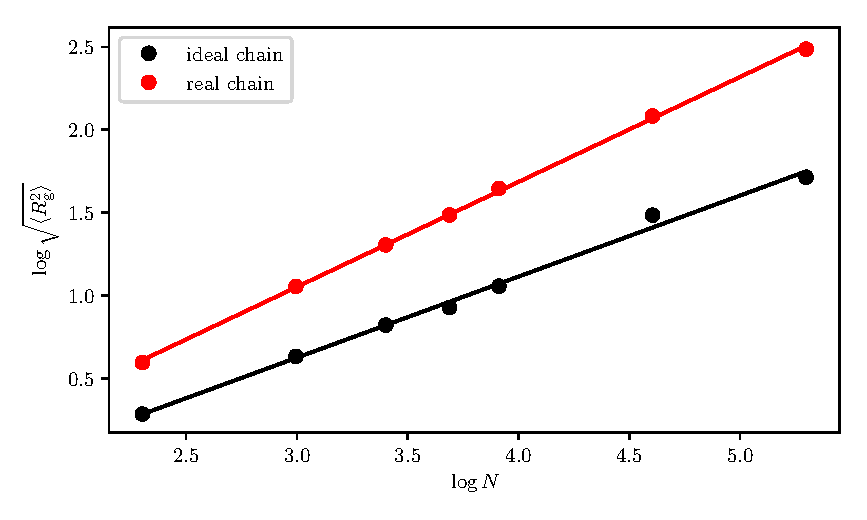
\includegraphics[width=\textwidth]{fit.pdf}
\caption{Log-log plot of the square root of the mean squared radius of gyration as a function of the number of monomers $N$ for an ideal chain (no excluded volume interaction) and a real chain (with excluded volume interaction). The markers indicate the values obtained from the ESPResSo simulations, the lines correspond to linear fits which were used to determine exponent $\nu$.}
\label{fig:fit}
\end{figure}

\subsection{Chain with Excluded Volume Interactions}
To simulate a real chain (with excluded volume interaction), we had to add a (purely repulsive) Lennard-Jones interaction between the monomers (this models the monomers as soft but repulsive spheres), this can be done in just a few additional lines of code:
\begin{lstlisting}
if args.with_LJ:
    system.non_bonded_inter[0, 0].lennard_jones.\\
    set_params(epsilon=lj1_eps, sigma=lj1_sig, cutoff=lj1_cut,\\
    shift='auto')
\end{lstlisting}
epsilon and sigma correspond to the parameters of the Lennard-Jones potential and cutoff is the radius beyond which the potential is set to zero. The shift option which is set to auto automically shifts the potential by a constant value such that there is no discontinuity which would lead to a Dirac-delta shaped force. The radius of gyration as a function of $N$ is shown in \autoref{fig:fit} (double log plot). From a linear fit, we get the exponent
\begin{align}
 \nu_\text{real chain} \approx 0.633.
\end{align}

\subsection*{Python Script for Fitting and Plotting}
For fitting and plotting we used the following Python script:
\begin{lstlisting}
import matplotlib.pyplot as plt
import numpy as np
from scipy.optimize import curve_fit

#Set plot size
width = 5.787
height = width*0.6
plt.rc('figure', figsize=(width,height))

#Use LaTeX for fonts
plt.rc('font',**{'family':'serif','serif':['Computer Modern']})
plt.rc('text', usetex=True)

dir_path = os.path.dirname(os.path.realpath(__file__))
dir_file = dir_path + '/gyration.csv'
N, rg2, rg2_lj = np.loadtxt(dir_file, delimiter =',',\\
unpack=False).T

#Fit
def fit(x, a, b):
    return a + b * x
param, cov = curve_fit(fit, np.log(N), np.log(np.sqrt(rg2)),\\
maxfev = 1000000)
print(param)

param2, cov2 = curve_fit(fit, np.log(N), np.log(np.sqrt(rg2_lj)),\\
maxfev = 1000000)
print(param2)

plt.plot(np.log(N), np.log(np.sqrt(rg2)), 'k', linestyle='none',\\
marker='o', label=r'ideal chain')
plt.plot(np.log(N), np.log(np.sqrt(rg2_lj)), 'r', linestyle='none',\\
marker='o', label=r'real chain')
plt.plot(np.log(N), fit(np.log(N), *param), 'k')
plt.plot(np.log(N), fit(np.log(N), *param2), 'r')

plt.xlabel(r'$\mathrm{log}\, N$')
plt.ylabel(r'$\mathrm{log}\,\\
\sqrt{\langle R_\mathrm{g}^2\rangle}$')
plt.legend()
plt.tight_layout()
plt.show()
\end{lstlisting}

\begin{thebibliography}{9}
		
		\bibitem{rubinstein}
		\textsc{M. Rubinstein} and \textsc{R. H. Colby},
		\emph{Polymer Physics},
		Oxford University Press,
		Oxford,
		2003.


\end{thebibliography}

\end{document}
